% !TEX encoding = UTF-8
% !TEX TS-program = pdflatex
% !TEX root = ../tesi.tex

%**************************************************************
\chapter{Progettazione e codifica}
\label{cap:progettazione-codifica}
%**************************************************************

\intro{Il capitolo approfondisce l’architettura e la codifica del software. Nella sezione 4.1 viene approfondita l'architettura e la logica del modulo, nella sezione 4.2 viene invece presentato l'iter seguito per la risoluzione dei problemi incontrati.}\\

\section{Architettura del modulo}

Il modulo è stato progettato tenendo a mente i requisiti di scalabilità imposti dall’azienda. L’architettura è stata definita durante le prime settimane e ha subito delle modifiche, anche in corso d’opera, in risposta ai bisogni ed alle difficoltà rilevate.

\subsection{Master e gestione degli url}

La gestione degli url ha come fulcro una coda \emph{Celery}, nella quale vengono immagazzinati gli url da analizzare. Il componente denominato ``master'' periodicamente inserisce nella coda url estratti da una lista stilata dall’analista. Il modulo ``worker'' preleva quindi gli url dalla coda assicurandosi di non averli già analizzati e tramite essi esegue la ricerca di nuovi url.  L'architettura in dettaglio della gestione degli url è rappresentata graficamente nella figura \ref{fig:architettura gestione url}.


\begin{figure}[!h] 
    \centering 
    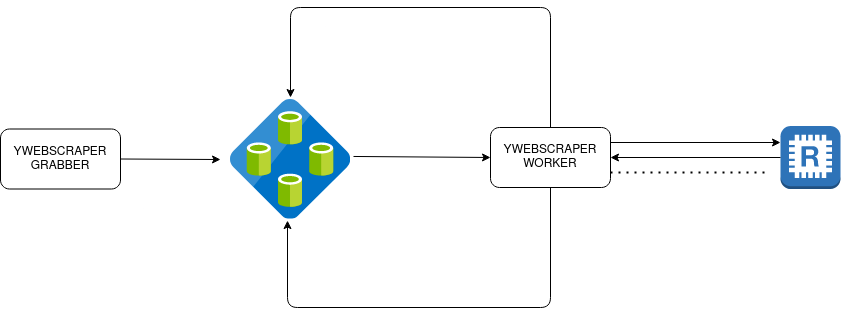
\includegraphics[width=1\columnwidth]{chapter4-project/architettura-gestione-url.png} 
    \caption{Architettura della gestione degli url in dettaglio}
    \label{fig:architettura gestione url}
\end{figure}
\newpage{}

\subsubsection{Ricerca nuovi url}
Una delle funzionalità del componente ``worker'' è l’estrazione degli url dalla coda \emph{Celery} e la loro analisi. Il primo controllo riguarda l’aver già analizzato in precedenza l’url estratto o meno. Se l’url non è presente nella cache di redis allora deve essere analizzato altrimento verrà scartato. Ad inizio analisi l’url viene inserito nella cache redis con un \gls{ttl} impostato dall’analista. Il worker quindi si occuperà di contattare il sito richiesto utilizzando il metodo specificato dall’analista e dal codice sorgente andrà ad estrarre e ripulire la lista di url. 


\subsubsection{Pulizia degli url}
Un url (\href{https://datatracker.ietf.org/doc/html/rfc1808.html#section-2.1}{da RFC 1808, Sezione 2.1}) è composto da \newline
\centerline{\texttt{<scheme>://<netloc>/<path>;<params>?<query>\#<fragment>}}
\newline
\begin{itemize}
	\item \textbf{scheme:} indica il protocollo utilizzato;
	\item \textbf{netloc:} \textit{ne}twork \textit{loc}ation, indica il dominio ed i sottodomini (se presenti), il numero di porta e opzionalmente le credenziali con la seguente sintassi: username:password;
	\item \textbf{path:} contiene informazioni sulla specifica risorsa alla quale accedere;
	\item \textbf{params:} campo opzionale contenente informazioni aggiuntive sul path, un esempio possono essere le informazioni aggiuntive da portare da una pagina alla successiva;
	\item \textbf{query:} campo opzionale contenente informazioni aggiuntive sul path, come da nome questo campo contiene le query;
	\item \textbf{fragment:} campo opzionale contenente informazioni aggiuntive sul path, un esempio possono essere i `\#’ che indicano in quale parte della risorsa portare la vista.
\end{itemize}
\noindent
Per realizzare una pulizia degli url completa serve fare le seguenti operazioni:
\begin{enumerate}
	\item per evitare di analizzare due pagine identiche con campi fragment differenti, viene eliminato il campo opzionale fragment;
	\item rendere tutti i caratteri nei campi scheme e netloc minuscoli;
	\item eliminazione di tutti gli url con contenuto nel campo scheme differente da http o https;
	\item aggiunta di http nel campo scheme in caso in cui sia vuoto;
	\item se l’url analizzato è relativo lo si trasforma in url assoluto;
	\item eliminazione di url uguali all’url iniziale inserito dal modulo ``master'', all’url precedente e all’url corrente;
	\item eliminazione degli url presenti nella lista di siti da non esplorare stilata dall’analista.
\end{enumerate}
Il codice che realizza la pulizia completa degli url è proposto nel listato \ref{listing: pulizia url}.

\begin{lstlisting}[caption=Pulizia completa dell'url.,
	label=listing: pulizia url]
	
    def _normalize_list_of_urls(self, url_list):
        normalized_url_set = set()
        for url in url_list:
            parse_url = urlparse(url)
            parse_url = self._clean_url(parse_url)
            # Url completo
            if parse_url.scheme == 'http' or parse_url.scheme == 'https' and parse_url.netloc:
                normalized_url_set.add(parse_url)
            # Mancanza solo di schema
            elif not parse_url.scheme and parse_url.netloc:
                parse_url = parse_url._replace(scheme='http')
                normalized_url_set.add(parse_url)
            # Relative url
            elif not (parse_url.scheme and parse_url.netloc) and parse_url.path:
                if parse_url.path == '/' or parse_url == '.':
                    parse_url = self.__site_url_parsed._replace(path='', params='', query='')
                else:
                    parse_url = self.__site_url_parsed._replace(path=parse_url.path,
                    	params=parse_url.params, query=parse_url.query)
                normalized_url_set.add(parse_url)
        return normalized_url_set	
	
    def _clean_url(self, url):
        # remove fragment, makes netloc and scheme lower case
        parse_url = url._replace(fragment='', scheme=url.scheme.lower(), 			   netloc=url.netloc.lower())
        return parse_url
        
        
    def _parse_valid_url_to_list(self, url_set: set) -> list:
        return_set = set()
        for url_parsed in url_set:
            if url_parsed:
                if url_parsed.path or url_parsed.params or url_parsed.query:
                    return_set.add(url_parsed.geturl())
                else:
                    netloc: str = url_parsed.netloc.lower()
                    if netloc.startswith('www.'):
                        netloc = netloc.split('www.', 1)[1]
                    if netloc.upper() not in SITE_BLACKLIST:
                        return_set.add(url_parsed.geturl())
        return list(return_set)
\end{lstlisting}


\subsubsection{Riprovare url}

L’analisi di alcuni url non andrà sempre a buon fine, per questo è stato necessario progettare una logica solida per ritentare il procedimento. Quando l’analisi di un url fallisce per qualsiasi motivo, esso viene reinserito nella coda contenente gli url da analizzare; all’url verrà assegnata una priorità minore, andando quindi ad inserirlo in fondo alla coda. Viene inoltre modificato il \gls{ttl} dell’url nella cache di \emph{Redis}, inserendo un \gls{ttl} minore, in modo che vengano ignorati per un breve lasso di tempo nuovi tentativi con lo stesso url non funzionante, così da non non sovraccaricare il server. Se lo stesso url viene riprovato n volte fallendo, con n scelto dall’analista, allora l’url viene scartato definitivamente. Il codice utilizzato per l'invio degli url da riprovare alla coda \emph{Celery}, viene riportato nel listato \ref{listing: Retry url}.

\begin{lstlisting}[caption=Invio degli url da riprovare alla coda.,
	label=listing: Retry url]
    def _push_to_retry_scraping(self, error: str = "") -> None:
        self.__obj_data['meta_info']['retry'] -= 1
        number_of_retry_left = 
            self.__obj_data['meta_info']['retry']
        if number_of_retry_left > 0:
            self.__obj_data['meta_info']['last_error'] = error
            self.__obj_data['meta_info']['timeout_value'] += 
                self.TIMEOUT_INCREMENT
            self.pushData(self.__obj_data, number_of_retry_left)
\end{lstlisting}


\subsection{Worker e ricerca di informazioni interessanti}

Il componente denominato ``worker'' oltre a gestire gli url andrà ad analizzare la pagina alla ricerca di informazioni considerate interessanti. Un grafico esplicativo della architettura ad alto livello è presente nella figura \ref{fig:architettura ricerca match}.
\begin{figure}[!h] 
    \centering 
    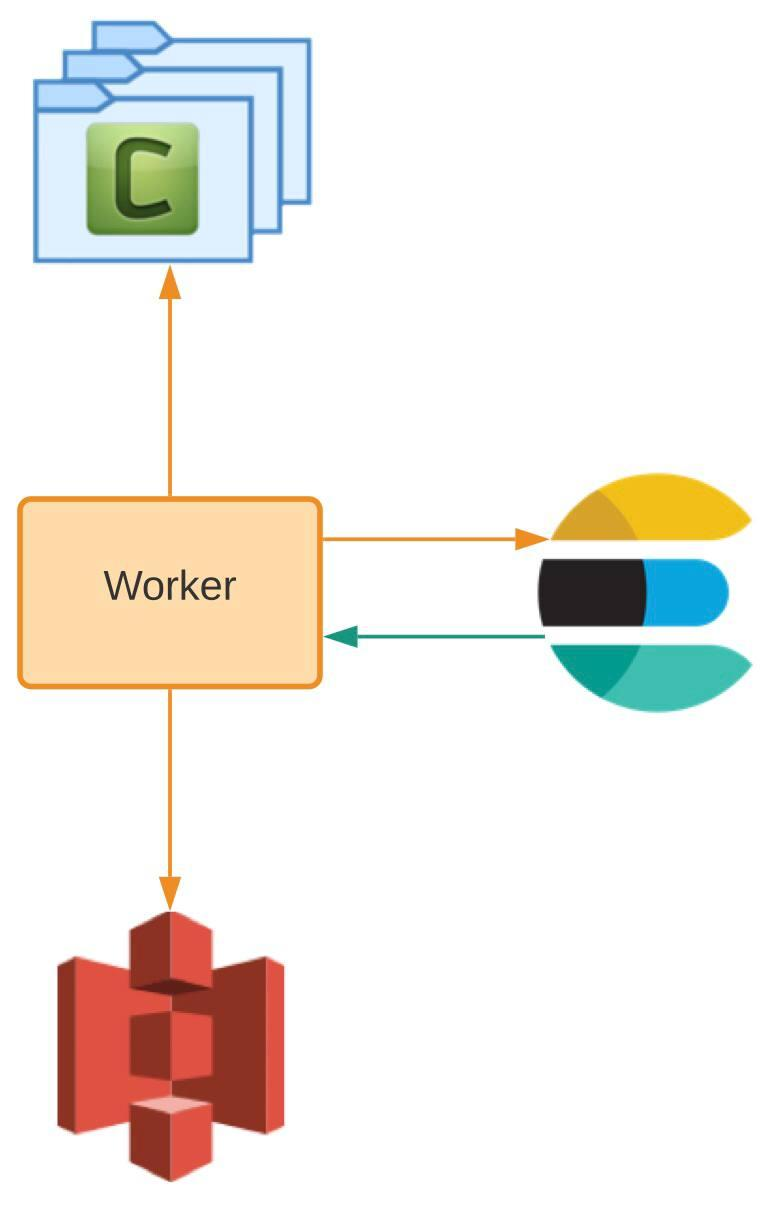
\includegraphics[width=0.35\columnwidth]{chapter4-project/architettura-match-search.png} 
    \caption{Architettura della ricerca di match in dettaglio}
    \label{fig:architettura ricerca match}
\end{figure}

\subsubsection{Ricerca informazioni interessanti}

La ricerca di informazioni interessanti avviene ricercando occorrenze sulla pagina html, tramite l’utilizzo di molteplici e complesse \emph{regex} stese dall’analista in precedenza. Queste \emph{regex} offrono un grado di granularità aggiuntivo poichè esse vengono sviluppate specificatamente per ogni azienda cliente. Il codice che esegue la ricerca tramite \emph{regex} è riportato nel listato \ref{listing: Ricerca tramite regex}. Se invece il contenuto del sito non è analizzabile, ad esempio un’immagine, allora viene analizzato l’\emph{header} restituito dal server. Quando vengono trovate occorrenze in un url si crea l’\emph{hash} della pagina tramite un algoritmo e viene controllato se l’\emph{hash} è presente su elasticsearch. Se non è presente allora viene mandato il sito con diverse informazioni aggiuntive nella coda \emph{Celery}. La coda è per un modulo differente presente nella infrastruttura, da questa coda infatti le informazioni vengono elaborate e se ritenute valide aggiunte ad \emph{Elasticsearch}. \newline{}
Se l’\emph{hash} non è presente su \emph{Elasticsearch} viene inoltre salvato il codice sorgente ed una istantanea della pagina su un \emph{bucket} di \emph{Amazon S3}. Il codice che effettua le operazioni di ricerca e salvataggio, descritte in precedenza, è presentato nel listato \ref{listing: Find match}

\begin{lstlisting}[caption=Ricerca tramite regex.,
	label=listing: Ricerca tramite regex]
    def _get_list_of_matches(self, search_inside: str) -> list:
        matches = list()
        # search for the regexes
        for regex in self.patterns:
            try:
                if regex.match(search_inside):
                    # we have a match, add to match list
                    matches.append(regex)
            except Exception as exmatch:
                logger.exception(exmatch, exc_info=True)
        return matches
\end{lstlisting}

\begin{lstlisting}[caption=Verifica della presenza delle informazioni su Elasticsearch ed opzionale aggiunta su Amazon S3 e ElasticSearch.,
	label=listing: Find match]
    obj_elastic = yfunctions.ElasticSearchData(self.__conf)
    res = obj_elastic.getData(hash_value=event_data['hash_value'])
    if res is None:
    	obj_event.pushData(store_data=False)
        s3 = yurlanalysis.YUrlAnalysis(self.browser)
        if self.is_save_screenshot_active:
        	s3.save_screenshot(event_data['hash_value'])
        if self.is_save_source_active:
			s3.save_page_source(event_data['hash_value'])
\end{lstlisting}
\newpage{}
\section{Risoluzione difficoltà incontrate}

Durante il progetto, sono state individuate e risolte diverse problematiche. Prenderemo in esempio uno dei problemi affrontati in modo da esporre il modus operandi per l’individuazione e risoluzione.
Ad ogni milestone settimanale raggiunta seguiva un periodo di test durante il quale il modulo operava e venivano raccolti diversi dati di diagnostica. Questi dati venivano poi studiati e verificato se risultassero in linea con le aspettative.

\subsection{Individuazione problema}
Durante la terza settimana di stage, avendo correttamente impostato i \emph{log} ed il codice, è stato possibile osservare i risultati delle prime run di test e la loro rappresentazione grafica mostrata in figura \ref{fig:test con memory leak}. Questi test hanno riportato dei dati estremamente diversi da quanto previsto. La memoria utilizzata cresceva sempre di più fino ad un arresto anomalo del programma dopo molte iterazioni. Questo tipo di problema viene chiamato ``\emph{memory leak}'', ovvero della memoria non viene liberata correttamente dal programma e rimane in utilizzo, accumulandosi.

\begin{figure}[!h] 
    \centering 
    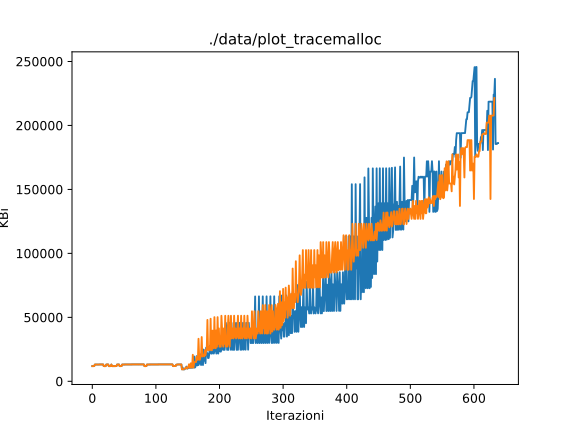
\includegraphics[width=0.8\columnwidth]{chapter4-project/test_con_memory_leak.png} 
    \caption{Test con memory leak}
    \label{fig:test con memory leak}
\end{figure}

\subsection{Lettura del grafico di memoria} \label{subsec:lettura grafico di memoria}
Nel grafico di memoria si hanno nella asse delle ascisse il numero di iterazioni eseguite durante il test (quindi indirettamente il tempo di esecuzione), mentre sull'asse delle ordinate si ha la memoria utilizzata in kibibyte (KiB). Sono presenti due funzioni per le due macchine che hanno eseguito i test in contemporanea: in blu viene rappresentato l'andamento della prima macchina di test mentre in arancione quello della seconda macchina di test.

\subsection{Risoluzione del memory leak}
Per la risoluzione del problema è stata prima effettuata una analisi del codice scritto, andando a stilare una lista di possibili problematiche collegate alla gestione della memoria. Una prima risoluzione delle problematiche legate al codice, non ha portato a miglioramenti nelle prestazioni. Per questo motivo è stata fatta una ricerca di problemi noti riguardanti le tecnologie utilizzate. Dalla ricerca è risultato che la libreria \emph{Celery}, con alcune specifiche impostazioni, non rilasciasse correttamente la memoria. Cambiando le impostazioni ed eseguendo una nuova run di test, si è potuto osservare nella figura \ref{fig:test senza memory leak} come la memoria venisse liberata correttamente. Per una legenda dettagliata del grafico fare riferimento a \ref{subsec:lettura grafico di memoria}.

\begin{figure}[!h] 
    \centering 
    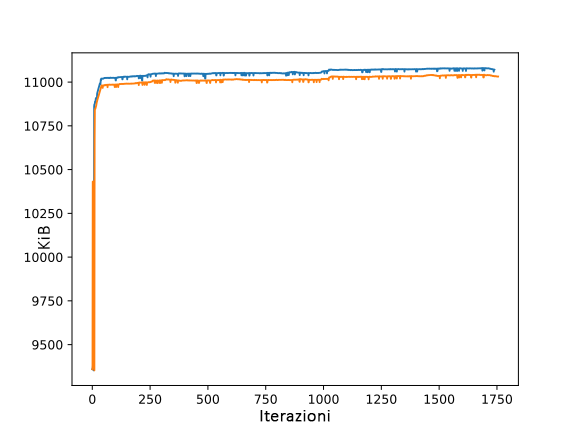
\includegraphics[width=0.8\columnwidth]{chapter4-project/test_senza_memory_leak.png} 
    \caption{Test senza memory leak}
    \label{fig:test senza memory leak}
\end{figure}